\section{AP Poisson}

\begin{frame}{Anitescu Potra (AP) Poisson Model \cite{APPoisson}}
\begin{itemize}
    \item Linear Complimentarity Problem (LCP) formulation for dynamic multi-body rigid contacts with friction
    \item Guarantees a solution to the contact problem
    \item Linearize the 3D friction model using a polyhedral cone (friction cone)
    \item Similar to the Wang Mason model, we optimized over the two input parameters $\mu$ and $\epsilon$
    \begin{figure}
        \centering
        \includegraphics[scale=0.25]{figures/linearFrictionCone.png}
        %\caption{Energy Ellipse\cite{nima2}}
        %\label{fig:frictionCone}
\end{figure}
    
\end{itemize}

\end{frame}

\subsection{Implementation and LCP Formulation}
\begin{frame}{Implementation and LCP Formulation \cite{ErlebenK}}

    Complimentarity Conditions (non-penetration, sliding velocity, and bounding frictional force) for linearized model:
    \begin{align*}
        0 \leq v_n \perp \lambda_n \geq 0 \\
        0 \leq \beta e + v_t \perp \lambda_t \geq 0 \\
        0 \leq (\mu\lambda_n-\sum_i \lambda_t_i) \perp \beta \geq  0 
    \end{align*}
    
    \begin{itemize}
        \item $v$ is contact velocity 
        \item $\lambda$ is contact impulse
        \item $t_i$ are unit vectors which positively span the frictional cone
        \item $\beta$ estimates maximum sliding velocity along $t_i$
    \end{itemize}
\end{frame}

\begin{frame}{Implementation and LCP Formulation \cite{ErlebenK}}
Writing the LCP in matrix form,
    \[
        0 \leq
        \underbrace{
        \left [
        \begin{array}{ccc}
             \textbf{B}_{nn} & \textbf{B}_{nt} & 0 \\
             \textbf{B}_{tn} & \textbf{B}_{tt} & e \\
             \mu & -e^T & 0 \\
        \end{array}
        \right ]
        }_{\text{A}}
        \underbrace{
        \left [
        \begin{array}{c}
            \lambda_n \\
            \lambda_t \\
            \beta   \\
        \end{array}
        \right ]
        }_\text{x}
        + \underbrace{\left [
        \begin{array}{c}
            \textbf{b}_n \\
            \textbf{b}_t \\
            0   \\
        \end{array}
        \right ] }_\text{b}
        \perp 
        \underbrace{\left [
        \begin{array}{c}
            \lambda_n \\
            \lambda_t \\
            \beta   \\
        \end{array}
        \right ]}_\text{x}
        \geq 0
    \]
    we can solve it using an implementation of Lemke's (pivoting) algorithm\\
    \begin{itemize}
        \item $\textbf{B}_{x_1x_2} = \textbf{J}_{x_1} \textbf{M}^{-1} \textbf{J}_{x_2}^T,\ \textbf{b}_{x_1} = \textbf{J}_{x_1} \textbf{M}^{-1} \textbf{F} $
        \item $\textbf{M}$ is the generalized mass matrix
        \item $\textbf{J}$ is the contact Jacobian
        \item $\textbf{F}$ is a vector containing external loads and gyroscopic forces
    \end{itemize}
\end{frame}


\begin{frame}{Implementation and LCP Formulation}
    \tikzstyle{startstop} = [rectangle, rounded corners, minimum width=3.5cm, minimum height=1.5cm, text centered, text width = 4cm, draw=black, node distance=3cm]
    \tikzstyle{arrow} = [ultra thick,->,>=stealth]
    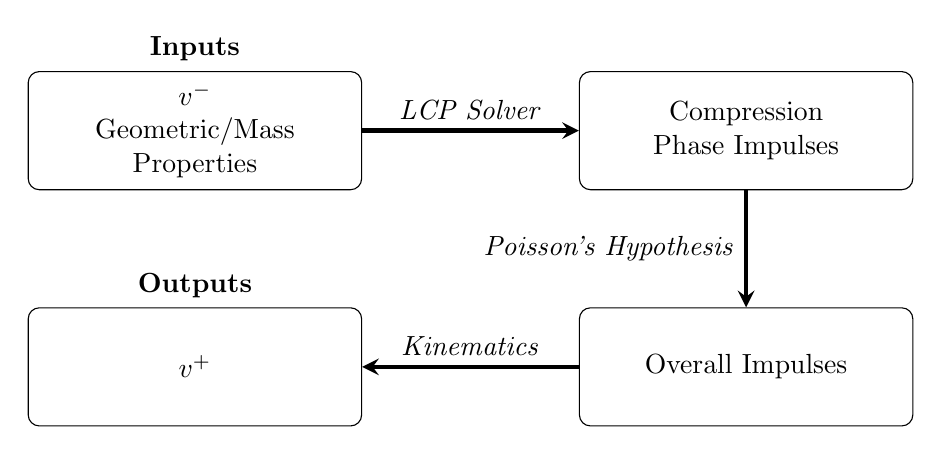
\begin{tikzpicture}[node distance=2cm]
        
            \node (in) [startstop, label=above:{\textbf{Inputs}}] { $v^-$ \\Geometric/Mass Properties \\ };
            \node (out)  [startstop, right of=in, node distance=7cm] {Compression Phase Impulses};
            \node (total)  [startstop, below of=out] {Overall Impulses};
            \node (final) [startstop, left of=total, , node distance=7cm, label=above:{\textbf{Outputs}}] { $v^+$};
            
            \draw [arrow] (in) -- (out) node[midway,above] {\textit{LCP Solver}};
            \draw [arrow] (out) -- (total) node[midway,left] {\textit{Poisson's Hypothesis}};
            \draw [arrow] (total) -- (final) node[midway,above] {\textit{Kinematics}};
    
    \end{tikzpicture}

    
\end{frame}


\subsection{Optimizing Parameters ($\mu$ and $\epsilon$)}

\begin{frame}{Optimal $\mu$ and $\epsilon$}
   \begin{itemize}
       \item Optimal $\mu$ : 0.089 (compared to 0.071 \cite{nima1} and 0.101 \cite{nima2})
       \item Optimal $\epsilon$ : 0.492 (compared to 0.568 \cite{nima1} and 0.526 \cite{nima2})
   \end{itemize}
 
\begin{figure}
    \centering
    \includegraphics[scale = 0.33]{figures/contour1000AP(UPDATED).jpg}
    \caption{Error contour plot for the AP Model}
    \label{fig:AP_contour}
\end{figure} 
    
\end{frame}

